\documentclass[xcolor=pdftex, x11names,table, oneside,11pt]{book}
%\usepackage{comment}
%\usepackage[utf8x]{inputenc}
%\usepackage[spanish, es-lcroman,es-tabla]{babel}
%\usepackage{amsmath}
%\usepackage{amsfonts}
%\usepackage{amssymb}
%\usepackage{graphicx}
\usepackage[letterpaper]{geometry}
\geometry{verbose,tmargin=2.5cm,bmargin=2.5cm,lmargin=3.5cm,rmargin=2.5cm}
%\setcounter{tocdepth}{3}
\usepackage{textcomp}
%\usepackage{amstext}
%\usepackage{setspace}
\usepackage[toc, page]{appendix}
\usepackage{tikz}
%\usetikzlibrary{arrows.meta}
%\usepackage{pgf}
%\usepackage{pgfplots}
%\usepgflibrary{decorations.pathmorphing}
\usepackage{xcolor}
\usepackage{tabulary}
\usepackage{colortbl}
%\usetikzlibrary{patterns}
%\usepackage{tikz-3dplot}
%\usepackage{etoolbox}
\usepackage{hyperref}
\usepackage{rotating}
\usepackage{float}
%\usepackage[section]{placeins}
\usepackage{afterpage}
%\usepackage{cleveref}
\usepackage{array}
%\usepackage{titlesec}
\usepackage{pdfpages}
\usepackage{hyperref}
%\usepackage[Sonny]{fncychap}
%\usepackage{caption}
%\usepackage[utopia]{quotchap}
%\hyphenation{de-sa-pa-ri-ci\'on}
%\onehalfspace
\usepackage{titletoc}
%\usepackage{titlesec}
\usepackage[shortlabels]{enumitem}
\usepackage{lipsum}
\hyphenation{trabajos}
%\titleformat*{\section*}{\color{c0}\normalfont\bfseries\LARGE}
\usepackage{booktabs}
\usepackage{multirow} 
\usepackage{multicol} 
\usepackage{adjustbox}
\usepackage[most]{tcolorbox}
\renewcommand{\arraystretch}{1.5}

%\usepackage{roboto}
%\usepackage{draftwatermark}
%\SetWatermarkText{\textbf{\textsc{EN REVISION}}}
%\SetWatermarkLightness{0.7}
%\SetWatermarkScale{2.5}
%\DraftwatermarkOptions{color={[rgb]{0.98, 0.91, 0.71}}}

%\newcommand{\art}[1]{{\section{Artículo \thesection  #1}}
\newcounter{articulo}
\refstepcounter{articulo}

\newcounter{capitulo}
\refstepcounter{capitulo}

\newcommand{\art}[1]{
\addcontentsline{toc}{section}{Art\'iculo \thearticulo. #1} 
\section*{Artículo \thearticulo: #1} 
\refstepcounter{articulo}
}

%%\addcontentsline{toc}{section}{Art\'iculo \thearticulo. Alcance}


\newcommand{\Chapter}[1]{
\addcontentsline{toc}{chapter}{Cap\'itulo \thecapitulo: #1} 
\chapter*{Cap\'itulo \thecapitulo: #1}
\refstepcounter{capitulo}
}

\definecolor{c1}{RGB}{143,85,69}
\definecolor{c2}{RGB}{218,37,39}
\definecolor{c3}{RGB}{231,121,25}
\definecolor{c4}{RGB}{247,215,75}
\definecolor{c5}{RGB}{0,146,64}
\definecolor{c6}{RGB}{0,141,221}
\definecolor{c7}{RGB}{153,71,121}
\definecolor{c8}{RGB}{171,169,169}
\definecolor{c9}{RGB}{255,255,255}
\definecolor{c0}{RGB}{0,0,0}
\definecolor{r1}{RGB}{246,205,162}
\definecolor{azul1}{RGB}{15,70,124}
\definecolor{azul2}{RGB}{63,108,150}
\definecolor{r2}{RGB}{232,54,67}
% \dottedcontents{<section>}[<left>]{<above-code>} {<label width>}{<leader width>}
\dottedcontents{chapter}[0em]{\addvspace{1pc} \bfseries}{1em}{1pc}%[\addvspace{1pc}]
\dottedcontents{section}[2em]{}{2em}{1pc}
\dottedcontents{subsection}[5em]{}{3em}{1pc}
\renewcommand{\contentsname}{\centering Contenidos}

\makeatletter

\usepackage{fancyhdr}
\pagestyle{fancy}
\pagestyle{myheadings}

\renewcommand{\appendixname}{Apéndices}
\renewcommand{\chaptername}{Cap\'itulo}

\renewcommand{\appendixtocname}{Apéndices}
\renewcommand{\appendixpagename}{Apéndices}
\newcommand{\itcr}{Instituto Tecnol\'ogico de Costa Rica}
\newcommand{\tfg}{Trabajo Final de Graduaci\'on}
\newcommand{\tfgs}{Trabajos Finales de Graduaci\'on}
\newcommand{\ef}{Escuela de F\'isica}
\newcommand{\ualif}{Unidad Acad\'emica de la Licenciatura en Ingenier\'ia F\'isica}
\newcommand{\cualif}{Consejo de \ualif}
\newcommand{\lif}{Licenciatura en Ingenier\'ia F\'isica}
\newcommand{\Def}[2]{\textbf{\texttt{#1:}}#2 \\[.25cm]}
%\newcommand{\Def}[2]{\begin{minipage}{\textwidth}\\ \texttt{#1:}#2  \end{minipage} }

\makeatletter
\renewenvironment{titlepage}
 {%
  \if@twocolumn
    \@restonecoltrue\onecolumn
  \else
    \@restonecolfalse\newpage
  \fi
  \thispagestyle{empty}%
 }
 {%
  \if@restonecol
    \twocolumn
  \else
    \newpage
  \fi
 }
 
%\titleformat{\chapter}[display]{\normalfont\huge\bfseries}{\chaptertitlename\ \thechapter}{0pt}{\Huge}

%\titleformat{\section}[box]{\Huge\bfseries}{-}{0pt}{\Huge\bfseries}

%\titlespacing*{\chapter}{0pt}{-1.5cm}{1cm}


\setcounter{secnumdepth}{3}
\setcounter{tocdepth}{3}

\hypersetup{
    colorlinks=true,
    linkcolor=blue,
    filecolor=magenta,      
    urlcolor=cyan,
    pdfpagemode=FullScreen,
    }

%glosario
%\makeglossaries
\setlength{\parindent}{0pt}

\makeatletter
\renewcommand{\@seccntformat}[1]{\llap{\textcolor{c1}{\csname the#1\endcsname}\hspace{1em}}}                    
\renewcommand{\section}{\@startsection{section}
{1}{0.9cm}%0.9 corre la numeraci�n hacia adentro
{-4ex \@plus -1ex \@minus -.4ex}
{1ex \@plus.2ex }
{\color{c6}\normalfont\Large\sffamily\bfseries}}
\renewcommand{\subsection}{\@startsection {subsection}{2}{\z@}
{-3ex \@plus -0.1ex \@minus -.4ex}
{0.5ex \@plus.2ex }
{\color{c2}\normalfont\large\sffamily\bfseries}}
\renewcommand{\subsubsection}{\@startsection {subsubsection}{3}{\z@}
{-2ex \@plus -0.1ex \@minus -.2ex}
{0.2ex \@plus.2ex }
{\color{c3}\normalfont\small\sffamily\bfseries}}                        
\renewcommand\paragraph{\@startsection{paragraph}{4}{\z@}
{-2ex \@plus-.2ex \@minus .2ex}
{0.1ex}
{\normalfont\small\sffamily\bfseries}}
\makeatother
% Fin numeraci�n secciones



%---------------------------------------------------------------------------------
%  Entornos:  Ejemplo, teorema, proposici�n, lema, lista de ejercicios, 
%             caja interludio, caja simple  
%---------------------------------------------------------------------------------

%  Cajas con el paquete  tcbcolor
%  CONTADORES: ejemplo, definicion, lema, teorema, corolario, proposicion,ejercicio 
\newcounter{tcbteo}[chapter]
\renewcommand{\thetcbteo}{\thechapter.\arabic{tcbteo}}

\newcounter{tcbdefi}[chapter]
\renewcommand{\thetcbdefi}{\thechapter.\arabic{tcbdefi}}

\newcounter{tcblema}[chapter]
\renewcommand{\thetcblema}{\thechapter.\arabic{tcblema}}

\newcounter{tcbcoro}[chapter]
\renewcommand{\thetcbcoro}{\thechapter.\arabic{tcbcoro}}

%  \newcounter{tcbListaEjercicios}[chapter]
%  \renewcommand{\thetcbListaEjercicios}{\thechapter.\arabic{tcbListaEjercicios}}

\newcounter{tcbpropo}[chapter]
\renewcommand{\thetcbpropo}{\thechapter.\arabic{tcbpropo}}

\newcounter{tcbvoca}[chapter]
\renewcommand{\thetcbvoca}{\thechapter.\arabic{tcbvoca}}

\newlength{\examlen}
\tikzset{
    wnodeTeorema/.style={%
         rectangle,  top color=gray!5, bottom color=gray!5,
         inner sep=1mm,anchor=west,font=\small\bf\sffamily},
   wnodeminimo/.style={%
         rectangle,  top color=white, bottom color=white,
         text=azulF,inner sep=1mm,anchor=west,font=\small\bf\sffamily}      
}

%\begin{teorema}  o \begin{teorema}[de tal] o \begin{teorema}[][ref]
% Teorema -----------------------------------------------------
\newtcolorbox{wwteorema}[2][]{%
arc=0mm,breakable,enhanced,colback=gray!5,boxrule=0pt,top=7mm,drop fuzzy shadow,
fontupper=\normalsize,step and label={tcbteo}{pink},
overlay unbroken = {\draw[color=pink,line width=0.2pt] (frame.north west)--([xshift=0pt]frame.north east);
%Caja de T�tulo: teo --
\node[wnodeTeorema](tituloteo) at ([xshift=0pt, yshift=-4mm]frame.north west)
{\textbf{\color{pink} #2}};
%Borde superior --
\draw[pink,line width=2.5cm] ([xshift=1.25cm, yshift=0cm]frame.north west)-- +(\examlen,3pt);
},%
overlay first = {\draw[color=pink,line width=0.2pt] (frame.north west)--([xshift=0pt]frame.north east);
%Caja de T�tulo: teo --
\node[wnodeTeorema](tituloteo) at ([xshift=0pt, yshift=-4mm]frame.north west)
{\textbf{\color{pink} #2}};
%Borde superior --
\draw[pink,line width=2.5cm] ([xshift=1.25cm, yshift=0cm]frame.north west)-- +(\examlen,3pt);
},%
% Mantener borde en cambio de p�gina 
overlay last = {\draw[color=pink,line width=0.2pt] (frame.south west)--([xshift=0pt]frame.south east);},
#1}
%-



\begin{document}
%\RaggedRight
\pagenumbering{roman}
%\urlstyle{rm} % Format style of \ur
%\thispagestyle{empty}
\thispagestyle{empty}
\setcounter{page}{0}
\begin{tikzpicture}
[   overlay,
    remember picture,
]
\fill[c1!10] (current page.north west)rectangle(current page.south east);
\fill[azul2] (current page.north west)-- (-5,-4)--(18,-1)--(current page.north east);
\fill[azul1] (current page.north west)-- (-5,-3)--(18,0)--(current page.north east);


\node[yshift=15ex, text width=\pdfpagewidth, align=center, above] (titulo) at (current page.center) {\fontsize{25}{30}\selectfont \textsc{Apuntes de Clase}};

\node[yshift=-5ex] (asignatura) [below of=titulo] {\fontsize{25}{30}\selectfont
\textsc{
\textcolor{azul1}{\textcolor{r2}{IF-6008} T\'opicos de Astronom\'ia y Astrof\'isica}}};

\node[yshift=-5ex] (profesor) [below of=asignatura] {\huge \texttt{Prof. Gerardo Lacy Mora}};

\node[above, yshift=20ex] (semestre) at (current page.south) {\texttt{I Semestre 2022}};

\node [below of=semestre] (lif){\texttt{Licenciatura en Ingenier\'ia F\'isica}};

\node [below of=lif] (ef){\texttt{Escuela de  F\'isica}};

\node[yshift=-10ex, xshift=-30ex] at (current page.north east) {
\includegraphics[width=7cm]{images/TEC.png}};

\end{tikzpicture}
	

\pagebreak


%\addcontentsline{toc}{chapter}{Índice general}
\thispagestyle{empty}
\tableofcontents



\pagebreak

\thispagestyle{empty}


%\texttt{¿De qué está hecho el universo? ¿C\'omo comenzo? ¿Cómo ha evolucionado durante los 13.800 millones de años desde su origen? ¿Y cómo terminará? Estas son las preguntas que aborda la cosmología, el estudio del universo en su conjunto. La investigación en cosmología involucra astronomía, pero también física gravitacional, física de partículas y preguntas desafiantes sobre la interpretación de fenómenos que no podemos ver directamente, como la posible existencia de algo antes del Big Bang.}
%\epigraph{
%\textbf{\textcolor{c2}{}}}}{\textsc{\href{https://www.cfa.harvard.edu/research/science-field/cosmology}{Center for Astrophysics // Harvard \& Smithsonian}}}
\begin{tikzpicture}[overlay,remember picture]
\node (centro) at (current page.center) {};
\fill[c1!10] (current page.west)rectangle(current page.south east);
\node (centro) at (current page.center) {};
\node[text width=\pdfpagewidth, below of=centro,yshift=-6ex] (hubble) {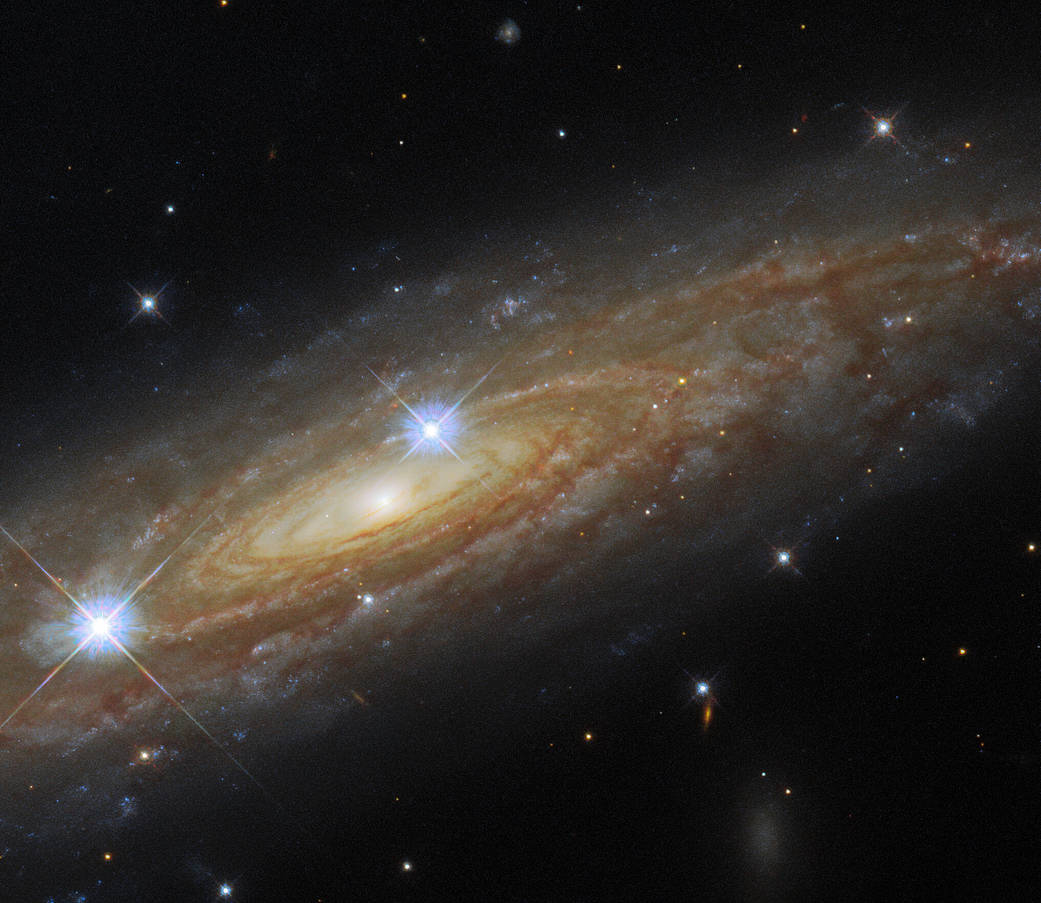
\includegraphics[width=\pdfpagewidth]{images/hubble_ugc11537_potw2146a.jpg}};
\node[text width=.9\pdfpagewidth,yshift=7ex] (cred) at (current page.south) {This image came from a set of observations designed to help astronomers weigh supermassive black holes in the centers of distant galaxies. Hubble’s sharp-eyed observations along with data from ground-based telescopes allowed astronomers to make detailed models of the mass and motions of stars in these galaxies, which in turn helps constrain the mass of supermassive black holes. Text credit: European Space Agency (ESA) Image credit: ESA/Hubble \& NASA, A. Seth};
\end{tikzpicture}
\pagebreak

\pagenumbering{arabic}

\section{Cosmolog\'ia y Galaxias}
%\begin{tikzpicture}[]
    % node definitions
    \node (s1) at (0, 0) {};
    \node (s2) at (1, 0) {};
    \node (s3) at (2, 0) {};
    \node (s4) at (3, 0) {};
    \node (s5) at (4, 0) {};
    % sketch
    \draw [test={1pt}{c1}{c2}, thick] (s1.center) to (s2.center);
    \draw [test={1pt}{c2}{c3}, thick] (s2.center) to (s3.center);
    \draw [test={1pt}{c3}{c4}, thick] (s3.center) to (s4.center);
    \draw [test={1pt}{c4}{c5}, thick] (s4.center) to (s5.center);
\end{tikzpicture}
%\section{Ley de Hubble}

%\section{Teoría del Big Bang}


\subsection{Cosmolog\'ia}

\begin{tikzpicture}[]
    % node definitions
    \node (s1) at (0, 0) {};
    \node (s2) at (1, 0) {};
    \node (s3) at (2, 0) {};
    \node (s4) at (3, 0) {};
    \node (s5) at (4, 0) {};
    % sketch
    \draw [test={1pt}{c1}{c2}, thick] (s1.center) to (s2.center);
    \draw [test={1pt}{c2}{c3}, thick] (s2.center) to (s3.center);
    \draw [test={1pt}{c3}{c4}, thick] (s3.center) to (s4.center);
    \draw [test={1pt}{c4}{c5}, thick] (s4.center) to (s5.center);
\end{tikzpicture}

La imagen que tenemos del Universo en el que vivimos ha estado fuertemente influida por dos \underline{observaciones} independientes:
\begin{itemize}
 \item La detección - inicialmente realizada por Arno Penzias y
Robert Woodrow Wilson en los años 60 \citep{penzias} - que el cielo est\'a lleno homogéneamente
de fotones de microondas, llamada \Textit{radiaci\'on de fondo -cósmico- de microondas} (CBM, por sus siglas en ingl\'es). Esta radiación corresponde a aquellos fotones que se dispersaron en una edad temprana
del Universo cuando las interacciones entre la luz y el plasma caliente que llenaba el espacio
se volvió insignificante\footnote{este periodo se conoce como \Textit{\'Epoca de recombinaci\'on}}.

\begin{figure}[!h]
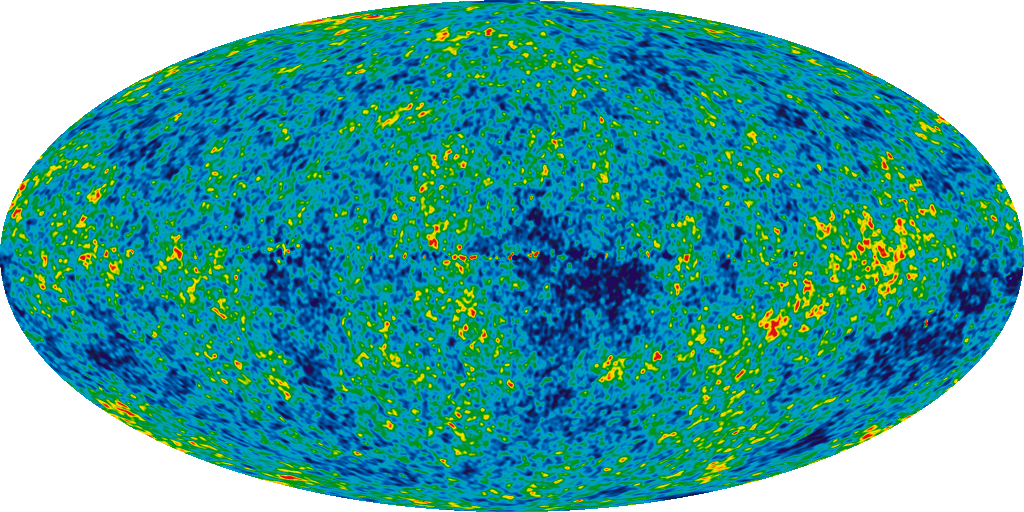
\includegraphics[width=\textwidth]{images/101080_7yrFullSky_WMAP_1024W.png}
\caption{The detailed, all-sky picture of the infant universe created from seven years of WMAP data. The image reveals 13.7 billion year old temperature fluctuations (shown as color differences) that correspond to the seeds that grew to become the galaxies. The signal from the our Galaxy was subtracted using the multi-frequency data. This image shows a temperature range of ± 200 microKelvin. Credit: NASA / WMAP Science Team}
\end{figure}

\item El otro gran descubrimiento en cosmología provino de la observación de que nuestro
universo se está expandiendo. Esto fue detectado inicialmente por Hubble (\citep{Hubble168}; \citep{hubblehumason1931}) basado en observaciones de variables cefeidas en varias nebulosas cercanas.

\begin{figure}[!h]
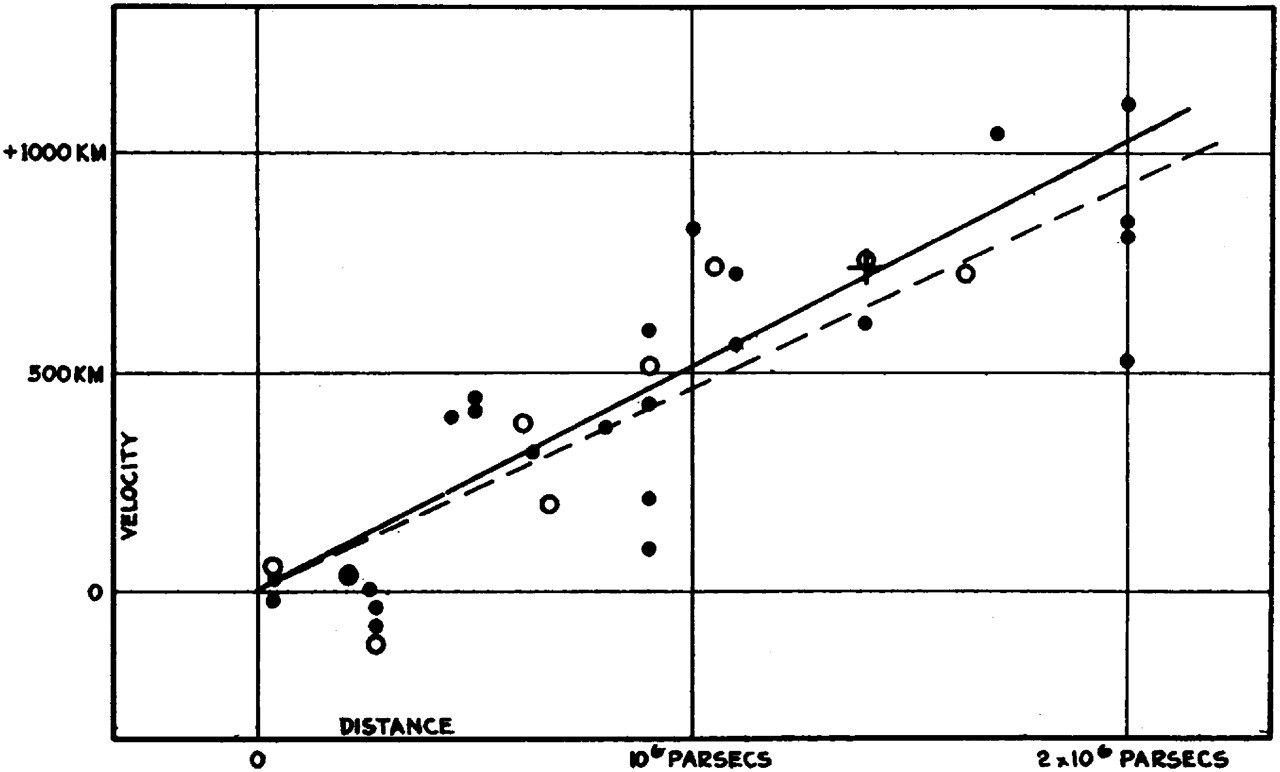
\includegraphics[width=\textwidth]{images/F2.large.jpg}
\caption{Hubble Law - Velocity-Distance Relation among Extra-Galactic Nebulae. Radial velocities, corrected for solar motion, are plotted against distances estimated from involved stars and mean luminosities of nebulae in a cluster. The black discs and full line represent the solution for solar motion using the nebulae individually; the circles and broken line represent the solution combining the nebulae into groups; the cross represents the mean velocity corresponding to the mean distance of 22 nebulae whose distances could not be estimated individually.}
\end{figure}

\end{itemize}


La expansión del Universo se ha confirmado a partir de observaciones de supernovas de tipo Ia (SNe
Ia)\footnote{SNe Ia son la fase explosiva de las enanas blancas que alcanzan el \Textit{límite de Chandrasekhar} despu\'es de acrecer masa de su compañero binario. Dadas las condiciones físicas de la explosión, la luminosidad producida
por la SN Ia se puede utilizar para medir la distancia a su galaxia anfitriona, raz\'on por la cual la SNs Ia se consideran como velas cosmológicas estándar.} (\citep{Riess_1998}; \citep{1999ApJ...517..565P}), que muestran que la expansión
en realidad, sucede a una tasa acelerada.  \\

Estos hechos implican que nuestro Universo era m\'as denso y caliente en el pasado (\Textit{Teor\'ia del Big Bang}). \\

La expansión del Universo est\'a asociada con la existencia de una energ\'ia de vac\'io,
generalmente referida como \Textit{Energía Oscura}. Según medidas de anisotrop\'ias del CMB ... \\

\begin{tikzpicture}[inner sep=4.5mm]
\node[fill, rectangle, c1] at (0,0) {};
\node[fill, rectangle, c2] at (1,0) {};
\node[fill, rectangle, c3] at (2,0) {};
\node[fill, rectangle, c4] at (3,0) {};
\node[fill, rectangle, c5] at (4,0) {};
\end{tikzpicture}

\subsection{Teor\'ia General de la Relatividad}
La cosmolog\'ia moderna se basa en la Teoría de la Relatividad General (TRG), propuesta por
Albert Einstein \citep{1917AE}, seg\'un el cual las propiedades geom\'etricas del espacio-tiempo
dependen de la distribución de materia y energ\'ia en el Universo. Dentro de TGR, las estructuras a grande escala que observamos hoy se formaron y evolucionaron (y est\'an evolucionando) a partir de 
inhomogeneidades en la distribución de masa del Universo primitivo que luego crecen bajo la influencia de la gravedad. \\

Estas ideas forman la base del \Textit{Modelo Cosmológico Estándar} ($\Lambda$-CDM\footnote{$\Lambda$-Cold Dark Matter}). \\

La Teor\'ia General de la Relatividad se basa en las \Textit{ecuaciones de campo de Einstein}:
\begin{equation}
R_{\mu \nu}-\frac{1}{2}g_{\mu \nu} R=\frac{8 \pi G}{c^4}T_{\mu \nu}-g_{\mu \nu}\Lambda,
\end{equation}
donde $R_{\mu \nu}$ (el tensor de curvatura de Ricci), $R$ (el escalar de curvatura) y $g_{\mu \nu}$ (el tensor m\'etrico) son t\'erminos relacionados con la geometr\'ia del espacio tiempo y $T_{\mu \nu}$ (el tensor de energ\'ia-esfuerzo) describe la densidad y flujo de energ\'ia y momentum en el espacio-tiempo; $c$ es la velocidad de la luz y $G$ es la constante gravitacional de Newton. El t\'ermino $\Lambda$ se llama \Textit{Constante Cosmol\'ogica} y representa la posibilidad de una densidad y presi\'on del vac\'io y/o que exista una rara forma de energ\'ia/materia gravitacional repulsiva, o Energ\'ia Oscura. \\

A partir de las mediciones de la radiaci\'on CBM, a largas escalas, el Universo puede considerarse espacialmente homeg\'eneo e isotr\'opico; en cuyo caso el tensor de energ\'ia-esfuerzo toma la forma de un fluido perfecto:

\begin{equation}
T_{\mu \nu}=(\rho + p)u_\mu u_\nu +pg_{\mu \nu},
\end{equation}

donde $\rho$ es la densidad de energ\'ia y $p$ es la presi\'on medida por un observador moviendose a 4-velocidad $u_\mu$. La densidda de energ\'ia suele escribirse como la contribuci\'on de cuatro fluidos posibles:

\begin{equation}
\rho=\sum \rho_i=\textcolor{c2}{\rho_m} + \textcolor{c5}{\rho_r} + \textcolor{c1}{\rho_\Lambda} + \textcolor{c3}{\rho_\kappa},
\end{equation}
donde $\textcolor{c2}{\rho_m}$,  $\textcolor{c5}{\rho_r}$, $\textcolor{c1}{\rho_\Lambda}$ y $\textcolor{c3}{\rho_\kappa}$ representan las contribuciones al presupuesto de densidad de energ\'ia de la materia, radiaci\'on, constante cosmol\'ogica y de la curvatura espacial, respectivamente. \\

El t\'ermino relacionado con la radiaci\'on usualmente se considera conformado por fotones CBM ($\rho_\gamma$) y neutrinos ($\rho_\nu$); mientras que la densidad de materia tiene aporte de materia bari\'onica ($\rho_{\Mbox{b}}$) y materia oscura fr\'ia ($\rho_{\Mbox{CDM}}$). \\

Una vez que se especifica el contenido de masa-energ\'ia del Universo, un modelo para la geometr\'ia del espacio-tiempo tiene que adoptarse para resolver las ecuaciones de campo de Einstein. Las m\'etrica de  Friemann-Roberson-Walker (FRW)

\begin{equation}
ds^2=-dt^2+a^2(t)\left[\frac{dr^2}{1-\kappa r^2}+r^2d\vartheta^2+r^2\sin^2\vartheta d\vartheta^2\right]
\end{equation}
es una soluci\'on exacta a las ecuaciones de campo de Einstein que describe todos los modelos isótropos, homogéneos,
uniformemente expandidos (o contra\'idos) del Universo. En la métrica FRW, $\kappa$
representa la curvatura espacial del universo y $a(t)$,  el \Textit{factor de escala}, representa la
expansi\'on relativa del universo. \\

Para un universo FRW, las ecuaciones de campo de Einstein pueden reducirse a dos ecuaciones independientes (\Textit{Ecuaciones de Friedmann}):


\begin{equation}
\frac{\dot{a}^2}{a^2}+\frac{\kappa c^2}{a^2}=\frac{8 \pi G}{3}\rho+\frac{\Lambda c^2}{3},
\end{equation}


\begin{equation}
\frac{\ddot{a}}{a}=-\frac{4 \pi G}{3} \left(\rho+\frac{3p}{c^2} \right)+\frac{\Lambda c^2}{3},
\end{equation}
donde $\dot{a}$ y $\ddot{a}$ representan la primera y segunda derivada temporal del factor de escala; respectivamente. \\

Para encontrar la evoluci\'on del factor de escala, se debe adoptar un modelo para la materia. En el caso de un universo FRW, es suficiente con establecer una \Textit{ecuaci\'on de estado}, es decir, $p=p(\rho)$; la cual puede parametrizarse como

\begin{equation}
p_i=\omega_i \rho_i c^2,
\end{equation}
donde el sub\'indice $i$ indica cada una de las posibles contribuciones al presupuesto de densidad de energ\'ia del universo. Para las componentes conocidas del Universo, $\omega_\gamma=\frac{1}{3}$, $\omega_{\Mbox{m}}=0$, $\omega_\kappa=-\frac{1}{3}$, $\omega_\Lambda=-1$ y $\omega_\nu$ est\'a en el rango $[0,\frac{1}{3}]$. \\

Si cada fluido se encuentra \Textit{desacoplado}, las ecuaciones de Friedmann se pueden combinar para expresar la evoluci\'on de la densidad de energ\'ia como
\begin{equation}
\dot{\rho_i}+3H(1+\omega_i)\rho_i,
\label{eq:ecF-d}
\end{equation}
donde $H$, el \Textit{par\'ametro de Hubble}, definido como

\begin{equation}
H\equiv H(t)\equiv \frac{da}{dt}\frac{1}{a},
\end{equation}
representa la tasa de expansi\'on del universo. El valor actual de $H$, denominado \Textit{constante de Hubble} suele normalizarse a la unidad, de manera que $H_0=H(t_0)=1$. Se acostumbra expresar la constante de Hubble en t\'ermino del \Textit{par\'ametro de Hubble adimensional} $h$, de manera que $H_0=100\, \textcolor{c1}{h} \,\mbox{km s}^{-1}\, \mbox{Mpc}^{-1},$\footnote{1 Mpc=$10^6$ pc = 3.086 $\times 10^{22}$ m. }
 y toda la incertidumbre en el valor de $H_0$ se asigna a $h$. \\
 
% 1 Mpc=$10^6$ pc = 3.086 $\times 10^{22}$ m.  \\
\citet{hubble0}

Una soluci\'on anal\'itica en el caso de que todas las componentes est\'en presentes no es posible,
pero para muchos casos de inter\'es es posible obtener soluciones anal\'iticas a la Ecuaci\'on \eqref{eq:ecF-d}.
Un resumen de tales soluciones se brinda en la Tabla 1. \\


La \Textit{densidad cr\'itica}, definida como
\begin{equation}
\rho_c\equiv \frac{3H^2}{8\pi G}
\end{equation}

es la densidad de energ\'ia que tendd\'ia un universo espacialemente plano ($\kappa=0$), sin constante cosmol\'ogica ($\Lambda=0$), con una tasa de expansi\'on $H(t)$. \\

El \Textit{par\'ametro de densidad} se define como

\begin{equation}
\Omega_i(t)\equiv \frac{\rho_i(t)}{\rho_c(t)}
\end{equation}
de donde 

\begin{equation}
\Omega=\Omega_m + \Omega_r + \Omega_\Lambda + \Omega_\kappa
\end{equation}

Un modelo cosmol\'ogico FRW se define especificando los valores de los tres par\'ametros cosmol\'ogicos $H_0$, $\Omega_{\Mbox{m}}$ y $\Omega_\Lambda$. \\

Los modelos FRW, al ser soluciones a universos homog\'eneos e isotr\'opicos, no permiten explicar la cantidad de estructuras en el universo. Para reproducir las \Textit{grandes estructuras} es necesario introducir inhomogeneidades iniciales en la densidad de energ\'ia que luego crecen bajo el efecto de la gravedad y gradientes de presi\'on en un universo en expansi\'on. Estas ``semillas'' se considera que fueron generadas a partir de fluctuaciones cu\'anticas, seguidas de una \'epoca de expansi\'on exponencial del universo temprano, denomida \Textit{inflaci\'on}. Las mediciones del CBM brindan restricciones observacionales a la forma de dichas pertubaciones iniciales de la densidad.\\

\begin{figure}
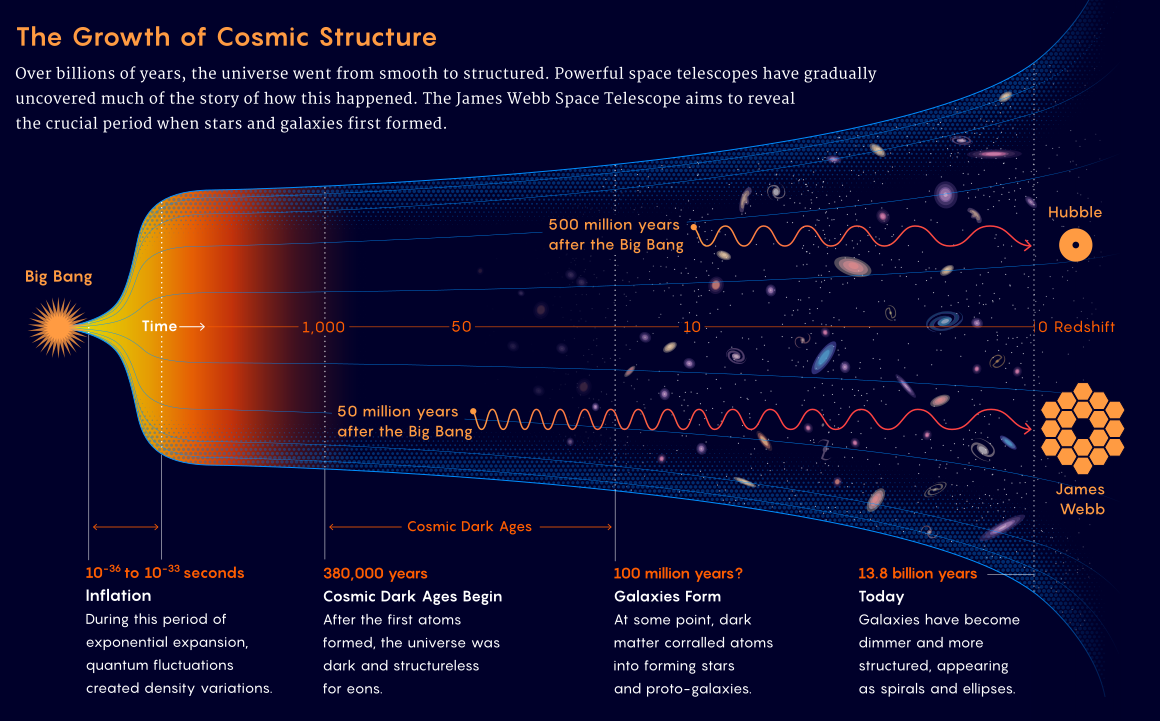
\includegraphics[width=\textwidth]{images/History-Universe-graphic.png}
\caption{El crecimiento de la estructura c\'osmica. Cr\'editos: Samuel Velasco (\href{https://www.quantamagazine.org/why-nasas-james-webb-space-telescope-matters-so-much-20211203/}{Quanta Magazine})}
\end{figure}


\subsection{Formación galáctica}

\begin{tikzpicture}[]
    % node definitions
    \node (s1) at (0, 0) {};
    \node (s2) at (1, 0) {};
    \node (s3) at (2, 0) {};
    \node (s4) at (3, 0) {};
    \node (s5) at (4, 0) {};
    % sketch
    \draw [test={1pt}{c1}{c2}, thick] (s1.center) to (s2.center);
    \draw [test={1pt}{c2}{c3}, thick] (s2.center) to (s3.center);
    \draw [test={1pt}{c3}{c4}, thick] (s3.center) to (s4.center);
    \draw [test={1pt}{c4}{c5}, thick] (s4.center) to (s5.center);
\end{tikzpicture}

La principal idea detr\'as de la teor\'ia de fomaci\'on de estructuras es que en un fluido homog\'eneo e isotr\'opico, pequeñas fluctuaciones en la densidad y velocidad pueden evolucionar en el tiempo si la escala temporal para que los efectos de la presi\'on se establezcan es mucho menor que la escala temporal necesaria para que dichas fluctuaciones en la densidad colapsen bajo el efecto de la gravedad. Bajo este esquema, se considera que las estructuras que observamos hoy d\'ia, se han formado jer\'arquicamente: pequeños halos (de materia oscura) se forman por colapso para formar halos m\'as grande que luego son el lugar de nacimiento de las galaxias. \\ 

\citep{ratra}

La \Textit{Teor\'ia de pertubaciones lineales} introduce pequeñas desviaciones a la homogeniedad e isotrop\'ia de una \Textit{m\'etrica FRW de fondo} para resolver las ecuaciones de Einstein. Las perturbaciones se caracterizan por un \Textit{funci\'on de contraste}, $\delta (\mathbf{x},t)$, de manera que las cantidades din\'amicas se pueden expresar como

\begin{equation}
\rho(\mathbf{x},t)=\bar{\rho}(t)[1 +\delta (\mathbf{x},t)],
\end{equation}

\begin{equation}
p(\mathbf{x},t)=\bar{p}(t)[1 +\delta (\mathbf{x},t)],
\end{equation}

donde $\bar{\rho}$ y $\bar{p}$ representan la densidad y presi\'on del campo de fondo; respectivamente. La teor\'ia de perturbaciones lineales es aplicable para $\delta \lesssim 1$. Luego, la evoluci\'on se vuelve no lineal. Si adem\'as se asumen pertubaciones adiab\'aticas, las fluctuaciones de densidad en un universo FRW dominado por materia crecen seg\'un\\ 

\begin{equation}
\frac{\partial^2\delta}{\partial t^2}+2H\frac{\partial\delta}{\partial t}=4\pi G \bar{\rho}\delta -\frac{c^2_{\mbox{s}}}{a^2}\nabla^2\delta,
\label{eq:densfluc}
\end{equation}
donde 

\begin{equation}
c^2_{\mbox{s}}\equiv \frac{\partial p}{\partial \rho}
\end{equation}
es la velocidad del sonido. Las derivadas temporales y el operador $\nabla$ operan sobre las \Textit{coordenadas com\'oviles}. \\

El segundo t\'ermino en \eqref{eq:densfluc} tiende a suprimir el crecimiento de las perturbaciones debidas a la expansi\'on del universo; por lo que suele llamarse \Textit{arrastre de Hubble}. El primer t\'ermino en el lado derecho de esta ecuaci\'on causa el crecimiento de las perturbaciones debido a inestabilidades gravitacionales, mientras que el segundo t\'ermino est\'a relacionado con la presi\'on debida  a variaciones espaciales de la densidad. \\ 

Dada la naturaleza lineal de la ecuaci\'on \eqref{eq:densfluc}, una expansi\'on en serie de Fourier 
\begin{equation}
\delta (\mathbf{x},t)=\sum_{\mbox{k}} \delta_{\mbox{k}}(t) e^{i \mbox{\textbf{k}} \cdot  \mbox{\textbf{x}}}
\end{equation}
permite estudiar la evoluci\'on de modos individuales; 
\begin{equation}
\ddot{\delta_k}+2H\dot{\delta_k}=-\omega_k^2\delta_k,
\label{eq:jeans}
\end{equation}
donde $\omega_k$ se define mediante la \Textit{relaci\'on de dispersi\'on}
\begin{equation}
\omega_k^2=\left(\frac{k c_s}{H} \right)^2-4\pi G \rho,
\end{equation}
con $k\equiv |\mathbf{k}|=2 \pi a/\lambda $ es el \Textit{n\'umero de onda comovil}. La ecuaci\'on \eqref{eq:jeans} representa un oscilador amortigado, llamada \Textit{ecuaci\'on de Jeans}, en la que el amortiguamiento proviene de la expansi\'on del universo y la pertubaci\'on de la densidad act\'ua como fuente. \\

La condici\'on $\omega_k^2=0$ establece la igualdad entre la presi\'on y las fuerzas gravitacionales, define una \Textit{longitud propia}
\begin{equation}
\lambda_J \equiv \frac{2 \pi a}{k_J}=c_s \sqrt{\frac{\pi}{G\bar{\rho}}}
\end{equation}
llamada \Textit{longitud de Jeans}. Perturbaciones bari\'onicas en escalas mayores a la longitud de Jeans no se ven afectadas por las fuerzas de presi\'on y pueden crecer; mientras que en escalas menores, pequeñas perturbaciones experimentan el efecto de los gradientes de presi\'on y oscilan como ondas ac\'usticas con amplitudes que crecen o decrecen exponencialmente. Por lo tanto, en el r\'egimen sub-Jeans, no hay crecimiento de estructuras en el r\'egimen lineal.


\subsection{Tipos de galaxias}

\begin{tikzpicture}[]
    % node definitions
    \node (s1) at (0, 0) {};
    \node (s2) at (1, 0) {};
    \node (s3) at (2, 0) {};
    \node (s4) at (3, 0) {};
    \node (s5) at (4, 0) {};
    % sketch
    \draw [test={1pt}{c1}{c2}, thick] (s1.center) to (s2.center);
    \draw [test={1pt}{c2}{c3}, thick] (s2.center) to (s3.center);
    \draw [test={1pt}{c3}{c4}, thick] (s3.center) to (s4.center);
    \draw [test={1pt}{c4}{c5}, thick] (s4.center) to (s5.center);
\end{tikzpicture}

\citet{peebles2021extended}

\citet{bag2021shape}

Las galaxias son los bloques de construcci\'on b\'asicos del Universo cuando se mira a las escalas m\'as grandes.
Estrictamente hablando, fueron observadas por primera vez por Sir Frederick William Herschel (1738-1822),
quien identific\'o una gran colección de objetos "nebulosos" en el cielo nocturno. Fue a partir de observaciones de Edwin Hubble (1889-1953) en la d\'ecada de 1920, que se estableci\'o claramente que esos
objetos se encontraban mucho m\'as all\'a de la V\'ia L\'actea (Hubble 1925). \\

Desde las primeras observaciones, pronto qued\'o claro que las galaxias tienen diferentes formas (morfolog\'ias)
y diferentes propiedades f\'isicas, situación que hoy en d\'ia se conoce como el \Textit{Zool\'ogico gal\'actico}. Esta diversidad hizo necesaria una "taxonomía de galaxias". La famosa \Textit{secuancia de Hubble} fue el primer esquema de clasificaci\'on morfol\'ogica consistente de galaxias, reuniendolas en 4 categor\'ias principales: el\'ipticas, lenticulares, espirales e irregulares. \\ 

\begin{itemize}
\item Las galaxias el\'ipticas (E) se caracterizan por tener isofotas casi elípticas
(contornos de brillo superficial constante). Se clasifican adem\'as como $En$ de acuerdo con
su elipticidad, donde $n$ es el entero m\'as cercano a $10(1 -b/a)$, donde $a$ y $b$ son las longitudes de su eje semimayor y semimenor, respectivamente. Emp\'iricamente, $n$
var\'ia entre 1 y 7. 
\item Las galaxias espirales (S) tienen presencia de brazos espirales alrededor
una estructura de disco delgado y una protuberancia central. Se subdividen en espirales normales y
espirales barradas (SB), seg\'un haya o no una estructura en forma de barra en
la parte central de la galaxia. A cada una de estas clases de espirales se le asignan adem\'as las letras
$a$, $b$ o $c$, seg\'un el brillo de la protuberancia en relaci\'on con el disco, lo compacto de
los brazos espirales alrededor de la galaxia y el grado en que es posible resolver las estrellas,
regiones HII y polvo en los brazos espirales. 
\item Las galaxias lenticulares (S0) son intermedias entre galaxias el\'ipticas y espirales, tienen una estructura similar a un disco, dominada por una protuberancia pero sin presencia de brazos espirales. En algunos casos, las galaxias lenticulares pueden tener una barra central, en cuyo caso se clasifican como SB0. 
\item las galaxias irregulares (Irr) son galaxias casi sin estructura perceptible (Irr I) o sin estructura (Irr II).
\end{itemize}

\begin{figure}[!h]
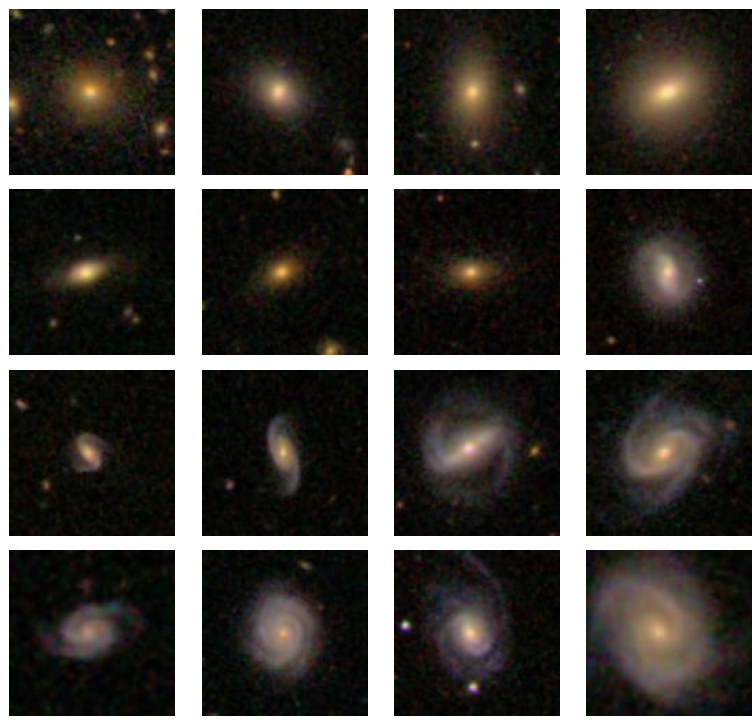
\includegraphics[width=\textwidth]{images/sdss-galaxies.png}
\caption{SDSS cutout images galaxies of diffeerent morphological type. From top to
bottom: Elliptical, Lenticular, Barred and Spiral galaxies. Each image is $48\times48\, \mbox{arcsec}^2 $}
\end{figure}


Incluso cuando la clasificaci\'on descrita anteriormente se bas\'o únicamente en la apariencia visual
de galaxias, hoy en d\'ia est\'a bien establecido que tal distinci\'on morfol\'ogica esta conectada a diferentes procesos f\'isicos y evolutivos subyacentes. Especialmente evidente de los estudios extragal\'acticos llevados a cabo a finales de los años 20 y principios de los 30 era el hecho que la distribuci\'on de las galaxias en el cielo no es uniforme sino que tienden a agruparse. \\


\begin{figure}[!h]
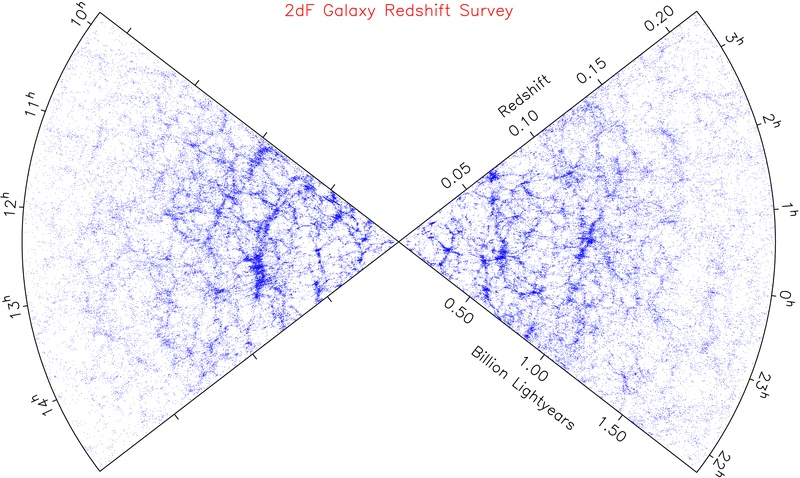
\includegraphics[width=\textwidth]{images/2dFzcone.jpg}
\caption{Galaxy distribution from the complete \href{http://magnum.anu.edu.au/~TDFgg}{2dFGRS}}
\end{figure}


Diferentes estudios en la d\'ecada de los años 80 comenzaron a encontrar fuertes correlaciones entre el tipo morfol\'ogico de las galaxias y sus ambientes. \\

El estudio de la distribuci\'on de las galaxias a gran escala y la dependencia de sus
propiedades en relaci\'on a su medio ambiente es uno de los principales objetivos de la cosmolog\'ia observacional. A partir de esta informaci\'on es posible establecer restricciones en los modelos cosmol\'ogicos. Esta es la raz\'on por la que cada vez se requieren estudios de galaxias más grandes y profundos. \\


As no single dark energy candidate or no particular modification of the theory of gravity is universally accepted as the right model to account for the alleged accelerated expansion of the universe, there is a recent trend of reconstructing the models for the observed universe through kinematical quantities \citep{DUARY2022101726}

\begin{tikzpicture}[inner sep=4.5mm]
\node[fill, rectangle, c1] at (0,0) {};
\node[fill, rectangle, c2] at (1,0) {};
\node[fill, rectangle, c3] at (2,0) {};
\node[fill, rectangle, c4] at (3,0) {};
\node[fill, rectangle, c5] at (4,0) {};
\end{tikzpicture}
\section{Enlaces de inter\'es}


\begin{wwteorema}{European Southern Observatory}
\href{https://www.eso.org/}{https://www.eso.org/}
\end{wwteorema}

\begin{wwteorema}{The Sloan Digital Sky Survey}
\href{https://www.sdss.org/}{https://www.sdss.org/}	

\end{wwteorema}

\begin{wwteorema}{Center for Astrophysics - Harvard \& Smithsonian}
\href{https://www.cfa.harvard.edu/research/science-field/cosmology}{https://www.cfa.harvard.edu/research/science-field/cosmology}
\end{wwteorema}

\begin{wwteorema}{Webb Space Telescope}
\href{https://www.jwst.nasa.gov/}{https://www.jwst.nasa.gov/}
\end{wwteorema}

\begin{wwteorema}{Astropy}
\href{https://www.astropy.org/}{https://www.astropy.org/}
\end{wwteorema}

\begin{wwteorema}{SciServer}
\href{https://www.sciserver.org/}{https://www.sciserver.org/} \\
\citep{sciserver}
\end{wwteorema}

\begin{wwteorema}{The Dark Energy Survey}
\href{https://www.darkenergysurvey.org/}{https://www.darkenergysurvey.org/}
\end{wwteorema}


\begin{wwteorema}{Marvin - the ultimate tool to visualise and analyse MaNGA data}
\href{https://dr17.sdss.org/marvin/}{https://dr17.sdss.org/marvin/}
\end{wwteorema}

\begin{wwteorema}{Hubble Space Telescope}
\href{https://hubblesite.org/}{https://hubblesite.org/}
\end{wwteorema}

\begin{wwteorema}{The SAO/NASA Astrophysics Data System}
\href{https://ui.adsabs.harvard.edu/}{https://ui.adsabs.harvard.edu/}
\end{wwteorema}

\begin{wwteorema}{Centre de Données astronomiques de Strasbourg - 
Strasbourg astronomical Data Center}
\href{https://cds.u-strasbg.fr/}{https://cds.u-strasbg.fr/} \\
\href{http://simbad.u-strasbg.fr/simbad/}{http://simbad.u-strasbg.fr/simbad/ \citet{simbad}}
\end{wwteorema}

\begin{wwteorema}{SAOImageDS9 - 
An image display and visualization tool for astronomical data}
\href{https://sites.google.com/cfa.harvard.edu/saoimageds9/}{https://sites.google.com/cfa.harvard.edu/saoimageds9/}
\end{wwteorema}

\begin{wwteorema}{The Millennium simulation}
\href{https://wwwmpa.mpa-garching.mpg.de/millennium/}{https://wwwmpa.mpa-garching.mpg.de/millennium/}
\end{wwteorema}

\begin{wwteorema}{The Stephen Hawking Centre for Theoretical Cosmology}
\href{https://www.ctc.cam.ac.uk/}{https://www.ctc.cam.ac.uk/}
\end{wwteorema}

\begin{wwteorema}{Astronomy and Computing}
\href{https://www.sciencedirect.com/journal/astronomy-and-computing}{https://www.sciencedirect.com/journal/astronomy-and-computing}
\end{wwteorema}

\begin{wwteorema}{Astronomy and Astrophysics}
\href{https://www.aanda.org/}{https://www.aanda.org/}
\end{wwteorema}

\begin{wwteorema}{Annual Review of Astronomy and Astrophysics}
\href{https://www.annualreviews.org/journal/astro}{https://www.annualreviews.org/journal/astro}
\end{wwteorema}

\begin{wwteorema}{Monthly Notices of the Royal Astronomy Society}
\href{https://academic.oup.com/mnras}{https://academic.oup.com/mnras}
\end{wwteorema}

\begin{wwteorema}{Gaia's stellar motion for the next 400 thousand years}
\href{ https://sci.esa.int/s/w5jGPMW }{ https://sci.esa.int/s/w5jGPMW }
\end{wwteorema}

\begin{wwteorema}{Journal of High Energy Astrophysics}
\href{https://www.sciencedirect.com/journal/journal-of-high-energy-astrophysics}{https://www.sciencedirect.com/journal/journal-of-high-energy-astrophysics}
\end{wwteorema}

\begin{wwteorema}{Living Reviews in Relativity}
\href{https://www.springer.com/journal/41114/}{https://www.springer.com/journal/41114/}
\end{wwteorema}



\pagebreak

\bibliography{bibliografia}{}






%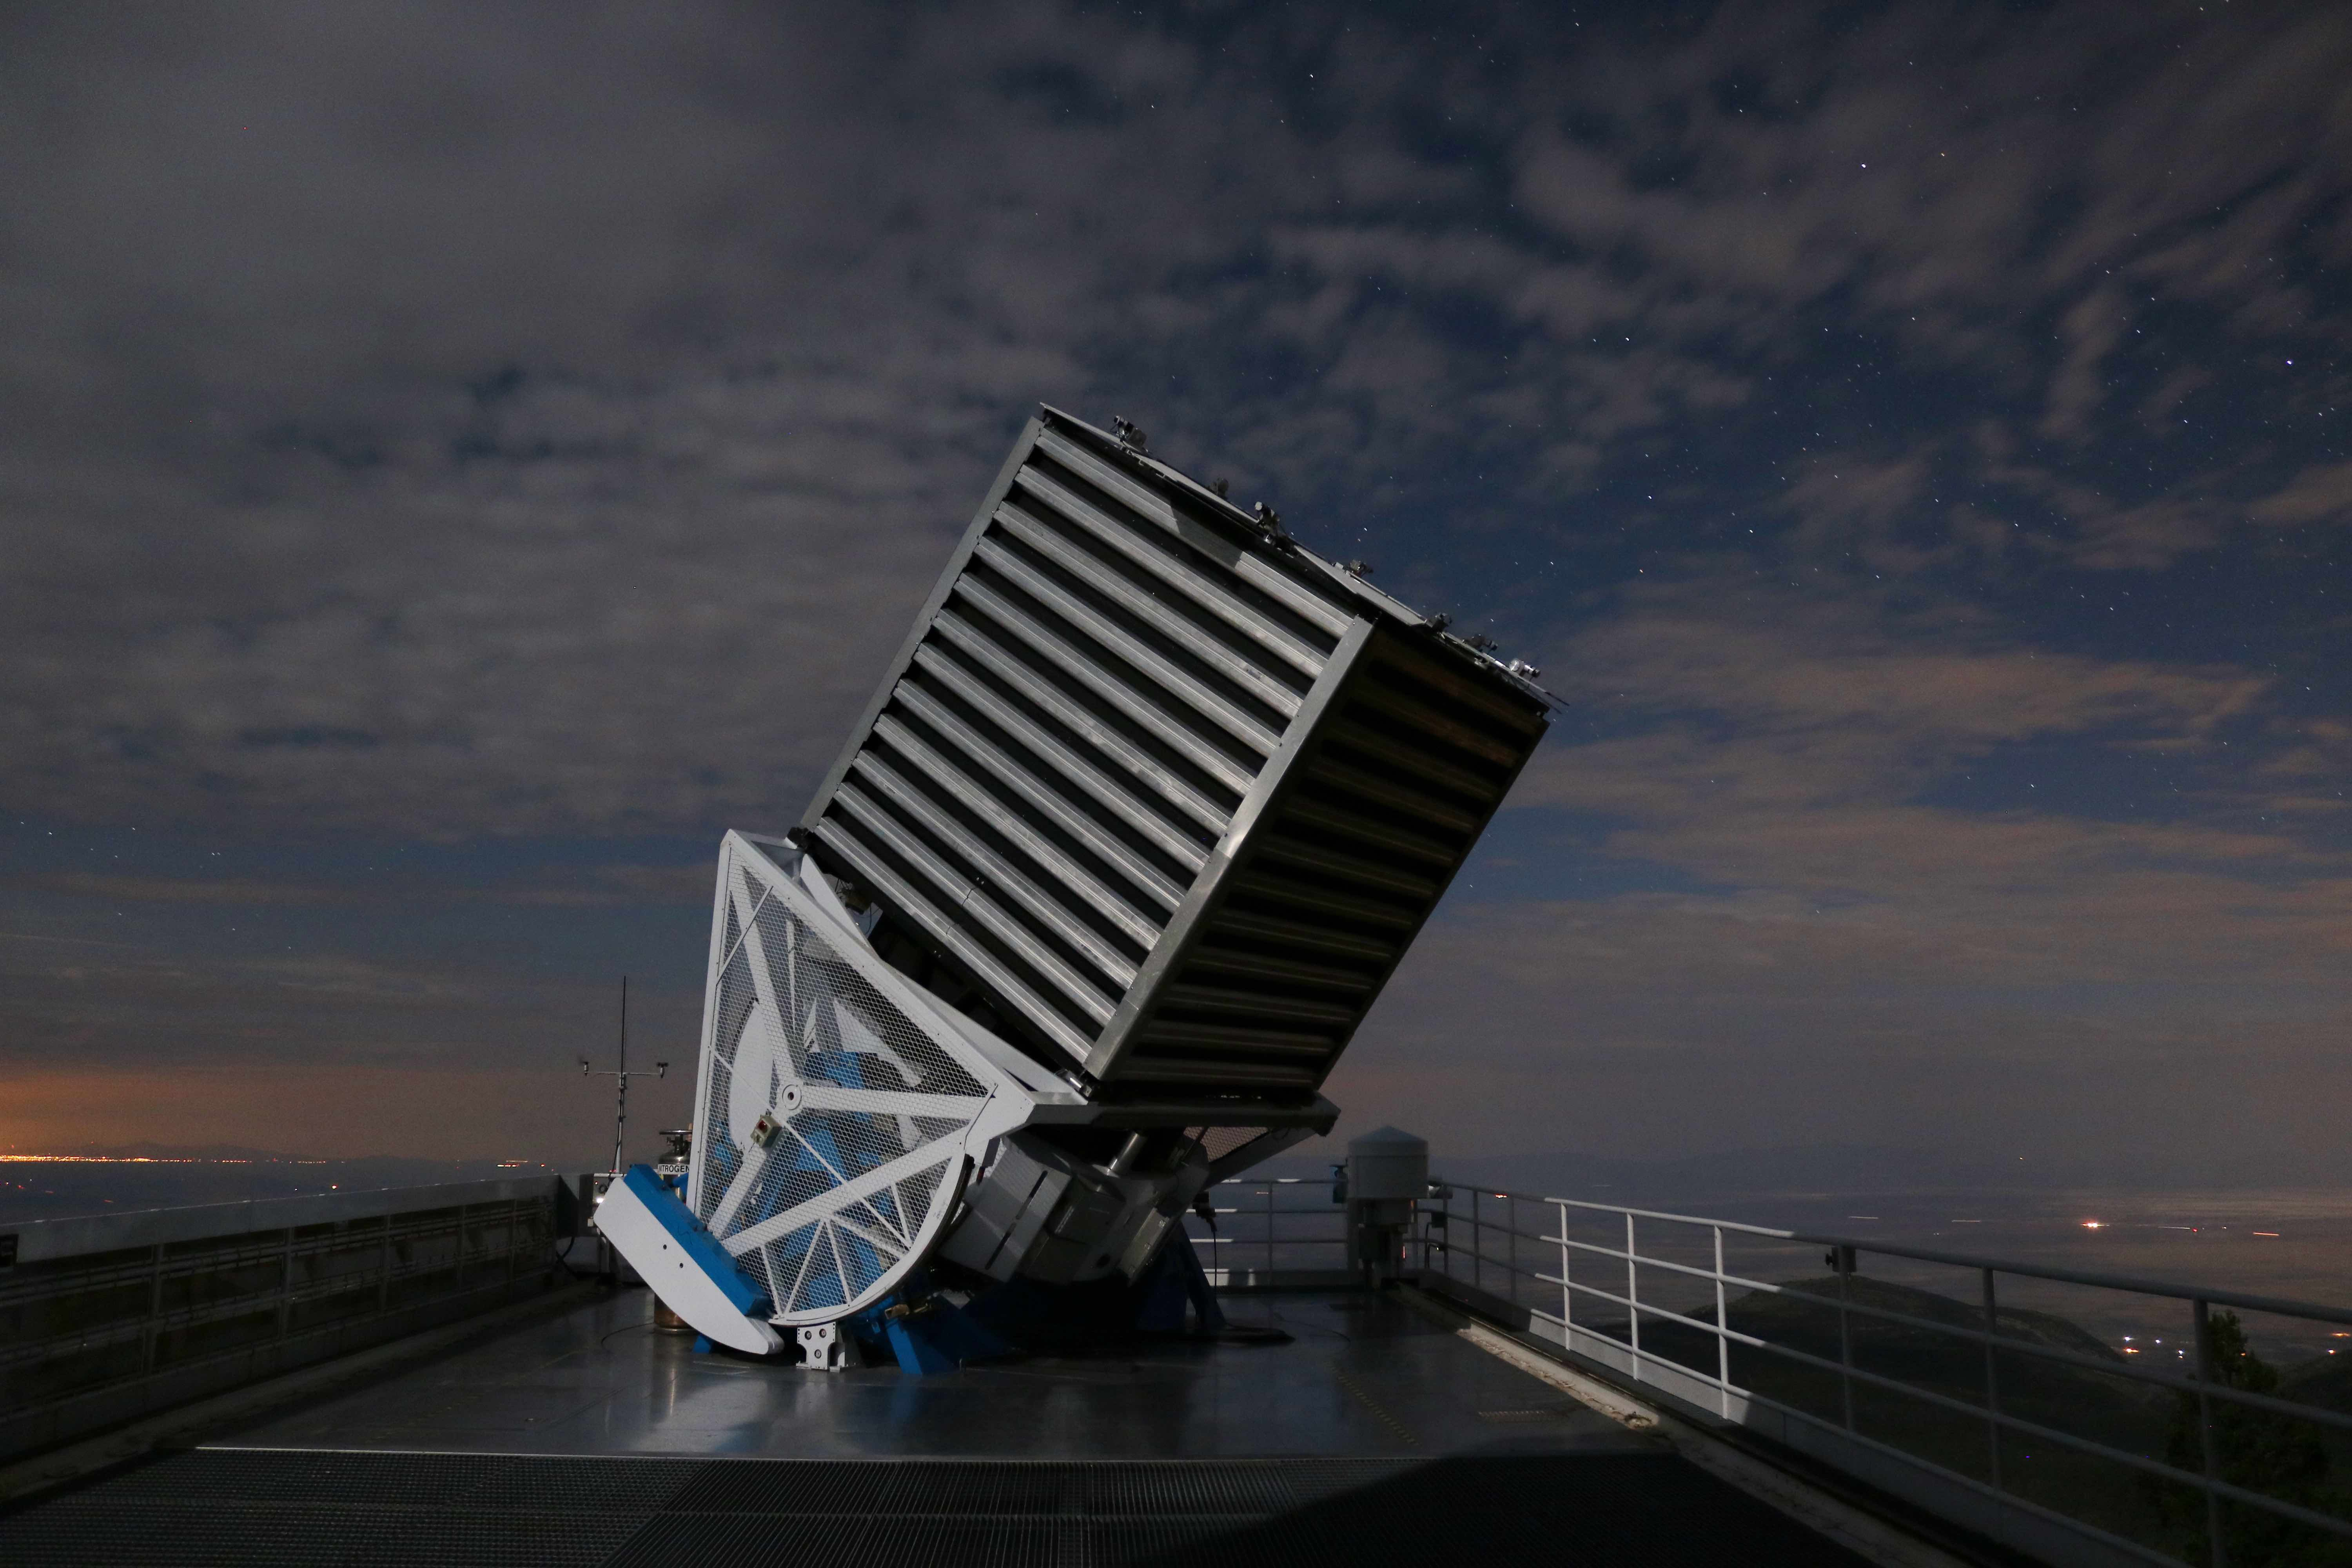
\includegraphics[width=.7\textwidth]{images/sdss_gaulme1.jpg}

%\begin{figure}
%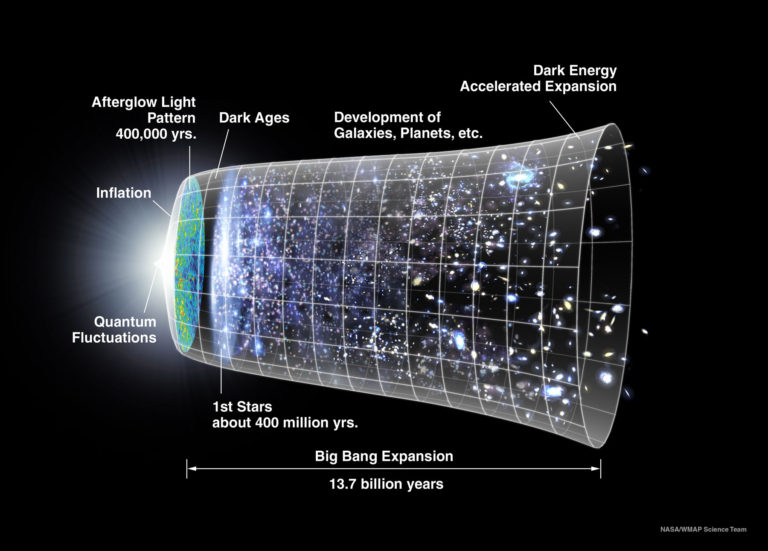
\includegraphics[width=.7\textwidth]{images/timeline-768x551.jpg}
%\caption{Timeline.}
%\end{figure}



%\bibliographystyle{apalike}



\begin{figure*}[b]
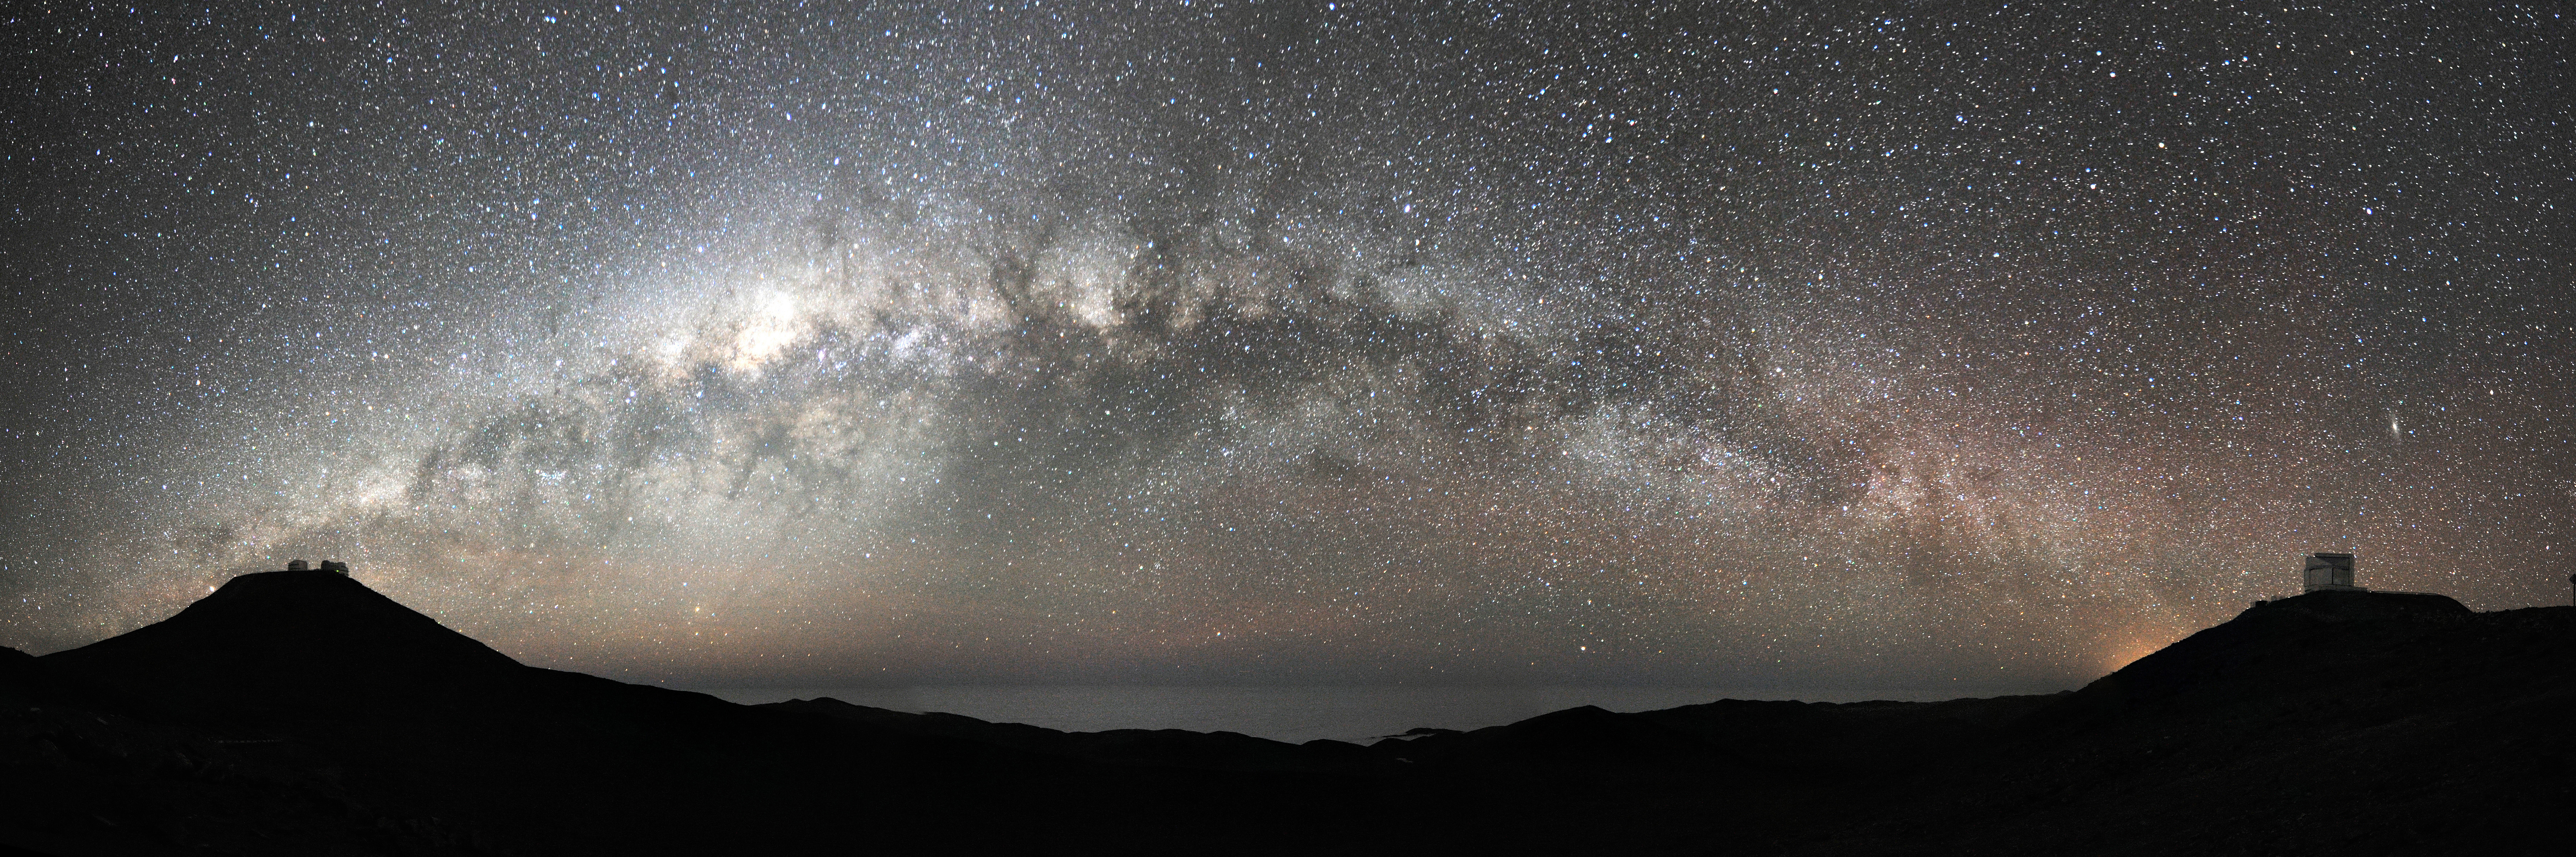
\includegraphics[width=\textwidth]{images/MW.jpg}
\caption{V\'ia L\'actea. Cr\'editos G. Hüdepohl (\href{https://www.atacamaphoto.com/}{atacamaphoto.com})/ESO}
\end{figure*}
\end{document}
